\documentclass[11pt]{article}
\usepackage[utf8]{inputenc}
\usepackage{amsmath}
\usepackage{listings}
\usepackage{xcolor}
\usepackage{booktabs}
\usepackage{geometry}
\usepackage{graphicx}
\usepackage{caption} % FIX: Added to support \captionof

\geometry{a4paper, margin=1in}

\definecolor{codegreen}{rgb}{0,0.6,0}
\definecolor{codegray}{rgb}{0.5,0.5,0.5}
\definecolor{codepurple}{rgb}{0.58,0,0.82}
\definecolor{backcolour}{rgb}{0.95,0.95,0.92}

\lstset{
    backgroundcolor=\color{backcolour},   
    commentstyle=\color{codegreen},
    keywordstyle=\color{magenta},
    numberstyle=\tiny\color{codegray},
    stringstyle=\color{codepurple},
    basicstyle=\ttfamily\small,
    breaklines=true,                 
    captionpos=b,                    
    keepspaces=true,                 
    numbers=left,                    
    numbersep=5pt,                  
    tabsize=2
}

\begin{document}

\title{Documentation: Logic Circuit Output Analysis (Q.12)}
\author{Digital Electronics Laboratory}
\date{}
\maketitle

\section{Step 1: The Question}
For the output $F$ to be $1$ in the logic circuit shown below, identify the correct input combination for $A$, $B$, and $C$.

\textbf{Options:}
\begin{itemize}
    \item (A) $A = 1, B = 1, C = 0$
    \item (B) $A = 1, B = 0, C = 0$
    \item (C) $A = 0, B = 1, C = 0$
    \item (D) $A = 0, B = 0, C = 1$
\end{itemize}

---

\section{Step 2: Logic Analysis}
The circuit evaluates inputs through XOR and XNOR stages:
\begin{enumerate}
    \item \textbf{Stage 1:} Inputs $A$ and $B$ produce $Y_1 = A \oplus B$ and $Y_2 = \overline{A \oplus B}$.
    \item \textbf{Stage 2:} Since $Y_1$ and $Y_2$ are complements, $Y_1 \oplus Y_2 = 1$.
    \item \textbf{Final Gate:} $F = \overline{Y_1 \oplus Y_2 \oplus C} = \overline{1 \oplus C} = C$.
\end{enumerate}

---

\section{Step 4: Graphical Output}
The graph below represents the logic level of $F$ as a function of the input combination index.

\vspace{0.5cm}
\begin{center}
    \begin{minipage}{0.8\textwidth}
        \centering
        % FIX: Using '2.png' from your file system and width=0.4 for small size
        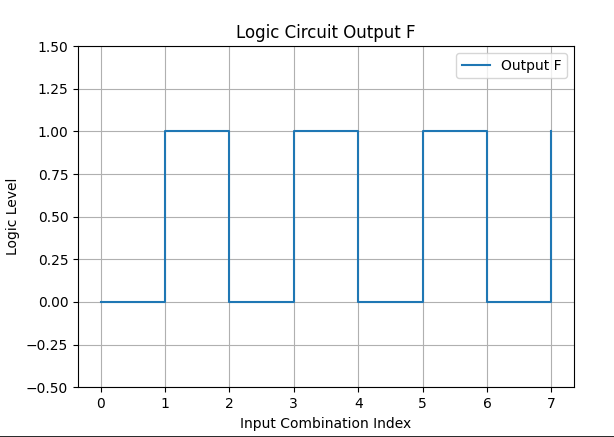
\includegraphics[width=0.4\textwidth]{2.png} 
        \captionof{figure}{Step plot showing $F=1$ at indices 1, 3, 5, and 7.}
    \end{minipage}
\end{center}
\vspace{0.5cm}

\section{Step 5: Final Result}
The output $F$ is high whenever $C=1$, confirming Option (D).

\textbf{Correct Match: (D) $A=0, B=0, C=1$}

\end{document}
